\documentclass[twoside,twocolumn]{article}
    \usepackage[a4paper, left=2cm, right=2cm]{geometry} % A4 paper size and thin margins
    \usepackage[sc]{mathpazo} % Use the Palatino font
    \usepackage[T1]{fontenc} % Use 8-bit encoding that has 256 glyphs
    \usepackage{microtype} % Slightly tweak font spacing for aesthetics
    \usepackage[english]{babel} % Language hyphenation and typographical rules
    \usepackage{booktabs} % Horizontal rules in tables
    \usepackage{enumitem} % Customized lists
    \usepackage[table,xcdraw]{xcolor}
    \usepackage[utf8]{inputenc} % Required for inputting international characters
    \usepackage{parskip}
    \usepackage{graphicx}
    \usepackage{hyperref}
    \usepackage{pdfpages}
    \usepackage{amsmath}
    \usepackage{esvect}
    \usepackage{listings}
    \usepackage{spverbatim}
    \usepackage[title]{appendix}
    \usepackage{subcaption}
    \hypersetup{
        colorlinks=true,
        linkcolor=blue,
        filecolor=magenta,      
        urlcolor=cyan,
    }
    \lstset{
        basicstyle=\ttfamily,
        frame=single
    }
    % Keywords
    \providecommand{\keywords}[1]
    {
        \small
        \textbf{\textit{Keywords---}} #1
    }

    \urlstyle{same}
    \setlength{\parindent}{18pt}
    \setlist[itemize]{noitemsep} % Make itemize lists more compact
    \makeatletter
    \newcommand*{\rom}[1]{\expandafter\@slowromancap\romannumeral #1@}
    \g@addto@macro{\UrlBreaks}{\UrlOrds}
    \makeatother

    \title{\LARGE \bf
    Optimization of Assignments for Teaching Assistants at UW
    }
    
    \author{ \parbox{3 in}{\centering Chongyi Xu, Weifan Jiang \\
             University of Washington\\
             MATH 381\\
             {\tt\small chongyix@uw.edu}\\{\tt\small wfjiang@uw.edu}}
    }

    \begin{document}
    \twocolumn[
        \maketitle
        \begin{@twocolumnfalse}
            \begin{abstract}
                For this project, we are focusing on developing a method to assign teaching-assistant candidates
                to different courses. Assigning candidates to their preferred teaching positions is important to 
                course coordinators at UW for a long time. Our purpose is to recommend a method of teaching-assistant
                assignments to solve this problem. We used simulated data to compare different methods that 
                we would use in the project. View \href{url}{https://github.com/weifanjiang/AssignTA} for our repository.
            \end{abstract}
            \keywords{Mathematical Model; Algorithm; Maximum Matching; Hungarian; Stable Marriage}
            \par\noindent\rule{\textwidth}{0.4pt}
        \end{@twocolumnfalse}
    ]
    %----------------------------------------------------------------------------------------
    %	ARTICLE CONTENTS
    %----------------------------------------------------------------------------------------


    \linespread{1.05} % Line spacing - Palatino needs more space between lines
    %------------------------------------------------
    \section{Problem Description}
    \indent The assignment of different teaching positions is a complicated task. The word "teaching position" 
    includes teaching assistants, graders and instructors here at UW. Each type of position has its 
    unique qualifications and requirments. Some positions require teaching, while other do not. 
    Most students are deemed to be certified to teach. Those whose first language is not English must 
    pass the SPEAK test to be certified. The position qualifications do not only appear in different roles 
    but also in different courses. For instance, the instructor positions would mostly be restricted to 
    graduate students or faculty. Meanwhile, the teaching assistant positions could open to both undergraduate students and 
    graduate students.
    \\ \indent The UW introduction courses to programming, such as CSE 142(Computer Programming I), are always popular. 
    There are over 700 students registered for around 50 sections each quarter. On the other hand, there are 
    also tiny-sized courses that designed for under 10 students. Therefore, the assignments of teaching positions 
    must satisfy the requirements for every single course each quarter such that everyone who registered for the course
    could have equal opportunity and fairly distributed teaching resources.   
    \\ \indent During the process of assignments, the course coordinators, who are in charge of assigning student candidates
    to appropriate roles, must consider the preference lists submitted by the candidates. Taking
    the example of UW CSE TA application form, as the candidates apply for CSE TA positions, they needs to choose their preferences 
    ("prefer not" or"neutral" or "prefer") for 12 distinct categories:
    \begin{itemize}
        \item AI and Robotics			
        \item Architecture			
        \item Computational Biology			
        \item Databases, Information Retrieval			
        \item Graphics, Vision, Animation			
        \item Hardware			
        \item Human-Computer Interaction			
        \item Introductory (CSE100,14x, 190)			
        \item Languages, Compilers, Software Engineering			
        \item Systems, Networks
        \item Theory			
        \item Uncategorize
    \end{itemize}
    \indent Following the information provided by CSE department, they initialize the preference value for each course that candidates prefer, 
    are neutral to, or prefer not to TA to 0.8, 0.5, and 0.2, respectively. This helps "push" candidates assignment towards courses 
    in areas they prefer and away from courses in areas they do not prefer. Without choosing preferences directly, candidates could establish
    their course preferences as well. If candidates choose to make up their own list, they would be asked to fill in a numerical number 
    between 0.0 and 1.0 that represents their preference to teach each courses that they are certified to TA. Besides preferences from 
    the candidates side, instructors preferences should also be considered. Instructors would be asked to fill in a form of preferred students.
    %------------------------------------------------
    \\ \indent Our motivation for the project is from the interview with undergraduate TAs and graduate TAs about their teaching experience in early quarters.
    (Hongtao Huang, hongth@cs.washington.edu, undergraduate teaching assistant at CSE; Tejas Devanur, tdevanur@uw.edu, graduate teaching fellow at Math Department
    ) They noticed that many times, even though they self-report their preferences, they got assigned to a course which 
    indicated as "less-preferred". Therefore, we would like to recommend a method that assigns candidates to
    courses, in such way that respects the following considerations:
    \begin{enumerate}
        \item Each candidate must be assigned to at most one course.
        \item Each course must be assigned an appropriate number of candidates.
        \item Each candidate must be assigned only to the courses for which they are qualified.
        \item Both candidates' and professors' preferences will be satisfied as much as possible.
    \end{enumerate}
    %------------------------------------------------
    \section{Simplification}
    In order to determine the best assignment that satisfy the above constraints, we will consider two things: what information is needed to
    find the optimal solution, and what assumption we need to make.
    \subsection{Input}
    \indent Below are the information needed to find the optimal solution:
    \begin{itemize}
        \item Preference of candidates for each role (grader, teaching assistant, instructor) for each course as numerical values between 0.0 and 
        1.0 where 0.0 indicates minimal preference and 1.0 indicates maximal preference.
        \item Qualification for each role for each course, which could be represented as an indicating matrix, where 1 entry indicates
        qualified for the role and 0 indicates not qualified.
        \item Preference of courses for each candidate to each role, which should also be a numerical value between 0.0 and 1.0 (larger indicates
        higher preference level).
        \item Capacity for each course (number of candidates needed for each role of any course, each course may differ).
    \end{itemize}
    %------------------------------------------------
    \subsection{Assumption}
    There were some assumptions we considered about in the draft phase
    \begin{enumerate}
        \item The quantifications were interpreted as qualifications. In other words, we would consider candidates' teaching experiences and GPA 
        as components of qualifications instead of quantifications. For instance, a no-teaching-experience candidate with GPA 
        less than $3.7$ would not consider to be qualified for the course he or she was applying for.
        \item Student candidates do not care about any factors other than their preferences, such as payment and work time.
        \item Candidate's time conflict with other courses they are taking is considered within qualifications.
        \item Student candidates will apply to all courses that they are qualified for. For those they are not interested in, they will give a 
        low preference.
        \item All candidates are legally registered UW students.
    \end{enumerate}
    For this project, we will ignore the need of other roles, and only focus on teaching assistant role. 
    %------------------------------------------------
    \section{Mathematical Model}
    Let $X = {x_1,...,x_m}$ represent $m$ student candidates, let $Y = {y_1,...,y_n}$ represent $n$ courses. \\
    Let $c_j$ represent the number of teaching assistants required for course $y_j$ for $1 \leq j \leq n$. \\
    Let $$q_{ij} = \begin{cases}1\text{, if $x_i$ is qualified to teach $y_j$} \\ 0\text{, otherwise} \end{cases}$$ \\
    The goal is to produce an assignment of candidates to courses, which should significantly consider the preference level of courses and candidates
    to each other. An assignment can be represented as 
    $$a_{ij} = \begin{cases}1\text{, if $x_i$ is assigned to $y_j$} \\ 0\text{, otherwise} \end{cases}\text{,}$$ 
    subject to the following hard constraints:
    \begin{enumerate}
        \item Each candidate must be assigned to at most one course: $$\forall x_i \in X, \sum_{j = 1}^n a_{ij} = 1\text{.}$$
        \item Each course must be assigned an appropriate number of candidates: $$\forall y_j \in Y, \sum_{i = 1}^m a_{ij} = c_j\text{.}$$
        \item Each candidate must be assigned only to the courses for which they are qualified: $$\forall x_j \in X,\ q_{ij} \geq a_{ij} \forall y_j \in Y\text{.}$$
    \end{enumerate}
    %------------------------------------------------
    \section{Solution of the Mathematical Problem}
    \subsection{Stable Marriage Algorithm}
    \indent In the field of computer science and mathematics, the stable match problem or stable marraige problem states that given N men and N women, 
    where each person has ranked all members of the opposite sex in order of preference, marry the men and women together such that there are no 
    2 people of opposite sex who would both rather have each other than their current partners. If there are no such people, all the marriages are “stable”.
    \\ \indent In 1962, D. Gale and L. S. Shapley, proved that, for any equal number of men and women, it is guaranteed
    that there is a stable matching. In their paper "College Admission and the Stability of Marriage", they defined the stability as following, an assignment
    of applications to colleges will be called unstable if there are two applicants $\alpha$ and $\beta$ who are assigned to colleges A and B, respectively,
    although $\beta$ prefers A to B and A prefers $\beta$ to $\alpha$. They considered a stable assignment to be optimal if every applicant is at least 
    as well off under it as under any other stable assignments.
    \\ 
    \begin{lstlisting}
*Gale-Shapley Algorithm*
INPUT: preference list for men and 
women
INITIALIZE matching set S to an empty 
set
WHILE (some woman w in W is still 
    unmatched and hasn't proposed 
    to every man in M)
    m <- first man on w's preference 
        list to whom w has not yet 
        proposed
    IF (m is unmatched)
        ADD pair (m, w) to S
    ELSE IF (m prefers w to existing 
            pair w')
        REPLACE (m, w') with (m, w) 
        FREE w'
    ELSE 
        w REJECT m
RETURN: matching S
    \end{lstlisting}
    \indent In this project, we have to slightly modify the algorithm in order to achieve our goal. Since each course may have need 
    of more than one candidate to be assigned, such changes will be made to the original Gale-Shapley Algorithm:
    \begin{enumerate}
        \item During each round of proposing, a currently unmatched candidate proposes to his/her top-choice course which he/she 
        has not proposed to yet.
        \item After candidates finish proposing to courses, each course takes the new proposers, put them into the same "set" with
        other candidates that are already matched with this course, to form a "temporary" waitlist.
        \item If the waitlist's length exceeds the course capacity, the waitlist will be sorted by course's preference to waitlist's
        members, and only the top $k$ ones will be kept, with $k$ being the capacity of that course.
        \item The algorithm terminates when there are no unmatched candidates or all candidates have proposed to all courses.
    \end{enumerate}
    \subsection{Hungarian Algorithm}
    The Hungarian Algorithm is a combinatorial optimization algorithm that solves the assignment problem in polynomial time.
    It was developed and published in 1955 by Harold Kuhn, who gave "Hungarian Algorithm" its name according to the previous works
    of two Hungarian mathematicians.
    \begin{lstlisting}
*Hungarian Algorithm*
INPUT: n*n cost matrix A
FOR EACH (row R_A in A)
    SUBTRACT min(R_A) from R_A
FOR EACH (column C_A in A)
    SUBTRACT min(C_A) from C_A
LABEL appropriate entries so that all
      zero entries are covered and 
      minimum number of labels are 
      used
IF (# labels = n)
    RETURN: labels as assignment    
ELSE:
    SUBTRACT min(A) from unlabeled 
              R_A
    ADD min(A) to unlabeled C_A
    REPEAT from LABEL
    \end{lstlisting}
    For this problem, the original Hungatian Algorithm has to be modified to be compatible with this problem:
    \begin{enumerate}
        \item The result of this problem is a many-to-one matching (multiple candidates assigned to one course). In order to 
        convert the problem to one-to-one matching, we will be splitting each course into slots (for example, if course A
        requires 5 candidates to be assigned, we will have 5 "slots" from A1 to A5, to corresponds to the 5 candidates wanted
        by A).
        \item Hungarian Algorithm also needs to run on a square matrix. We assume that there will always be more candidates than
        slots (if not, the department will need to advertise more to get more student apply as candidate). Thus, we can add
        "dummy" slots to make number of candidates and number of slots equal to each other. If a candidate matches to one of the
        dummy slots, this candidate is unselected for the row of teaching assistant.
        \item A "cost matrix" needs to be constructed for Hungarian Algorithm, and optimal solution (which is the output of
        Hungarian Algorithm) has minimized total cost. We let the row of cost matrix to be candidates, and column be the slots.
        Therefore, the value of $(i. j)$ should be:
        \begin{itemize}
            \item if $j$ is a "dummy" slot, then $(i, j)$ should be $0$ regardless of $i$. We need all "dummy" slots to have
            the same value, so the optimality if all "non-dummy" matches are not influenced by the dummy variables.
            \item if $i$ is not qualified to teach $j$, the value of $(i, j)$ should be infinity, therefore the Hungarian algorithm
            will avoid large cost and not choosing the unqualified entry. If the output assignment's cost is infinity, it indicates
            that no possible matching is available.
            \item If $i$ qualified to teach $j$, the $(i, j)$ entry should be $2 - \text{i's preference to j} - \text{j's preference to i}$
            therefore the cost is smaller if the sum of preference of candidate and course to each other is larger.
        \end{itemize}
    \end{enumerate}
    After making such modifications, Hungarian's algorithm will output an assignment of candidates to slots, which can be
    transferred to an assignment of candidates to courses. The sum of preferences to each other for all matched pair of
    candidates and courses is maximized.
    \subsection{Maximum Matching Algorithm}
    Consider an undirected graph $G=(V,E)$. A matching M is said to be maximal if M is not properly contained in any other matching.
    Formally, $M\notin M^{'}$ for any matching $M^{'}$ of $G$. Intuitively, this is equivalent to saying that a matching is maximal 
    if we cannot add any edge to the existing set. And a matching $M$ is said to be Maximum if for any other matching $M^{'}$, 
    $|M|\geq |M^{'}|$. Generally, maximum matching applied to unweighted graph more but for this project,
    we would like to modify the algorithm with weights in order to meet our propose. With researching, we will implement the method
    introduced by \textit{Zvi Galil}, Department of Computer Science, Columbia University, in 1986. In his study "Efficient Algorithms
    for Maximum Matching in Graphs", he developed this method based on Berge's Theorem, "the matching M has maximum cardinality if and 
    only if there is no augmenting path with respect to M."

    \indent Given a graph, $G=(V,E)$ and a matching $M \subset E$, a path $P$ is called an augmenting path for $M$ if:
    \begin{itemize}
        \item The two end points of $P$ are unmatched by $M$
        \item The edges of P alternate between edges $\in M$ and edges $\notin M$.
    \end{itemize}
    
    \begin{lstlisting}
*Maximum Matching*
INPUT: Graph G
M <- random selected matching
WHILE (there is a blossom and there 
       is an augmenting path in M)
    GROW the forest, labeling the 
         vertices even/odd
    IF (there is a blossom in the 
        graph)
        SHRINK the blossom to obtain 
               a new graph G'
        CONTINUE foresting
    ELSE
        FIND such even - even edges 
             to obtain a maximally 
             disjoint set of 
             augmenting paths 
             (P1,...,Pk)
    M <- switching edges along P's 
         from in-to-out of M and 
         vice-versa
EXPAND all blossoms to obtain the 
       maximum matching in the 
       original graph G.

    \end{lstlisting}
    
    In order to fit Maximum Matching algorithm to our model, we decide to construct a bipartite graph utilizing the data 
    we are working with. The first group of vertices will be implemented as distinct candidates, say, candidate group. 
    And the other group of vertices will be the courses we are assigning to, say, course group. Meanwhile, it has to be 
    considered that for each course in the course group, there is a required number of candidates they are looking for. 
    So we will modify our construction as the following:
    \begin{itemize}
        \item For each course $y_j \in Y$ in the course group, get the required number of candidates $c_j$.
        \item Construct a vertexc representing course $y_j$. And then make $c_j$ copies of the same vertex denoted as $y_j^k$.
        $1\leq k\leq c_j$.
        \item For each candidate $x_i\in X$, connect $x_i$ with all $y_j^k$ for which $x_i$ is qualified for.
        \item Weight the edge with a preference score $s = \lambda_1 p_{ij} + \lambda_2 p_{ji}$, where $\lambda_1=$ the weight of 
        candidates' preferences, $p_{ij}=$ candidate $x_i$'s preference to course $y_j$, $\lambda_2=$ the weight of 
        courses' preferences, $p_{ji}=$ course $y_j$'s preference to candidate $x_i$.  And for most cases, we are weighting
        courses' preferences and candidates' preferences equally. In the other word, $\lambda_1=\lambda_2=1$.
    \end{itemize}
    \textbf{Note:} When we say "courses' preferences", we are basically indicating the list submit by the professor(or instructor) 
    teaching that course, ranking his or her preferences to the candidates who are applying for that course.
    \begin{figure*}
        \centering
        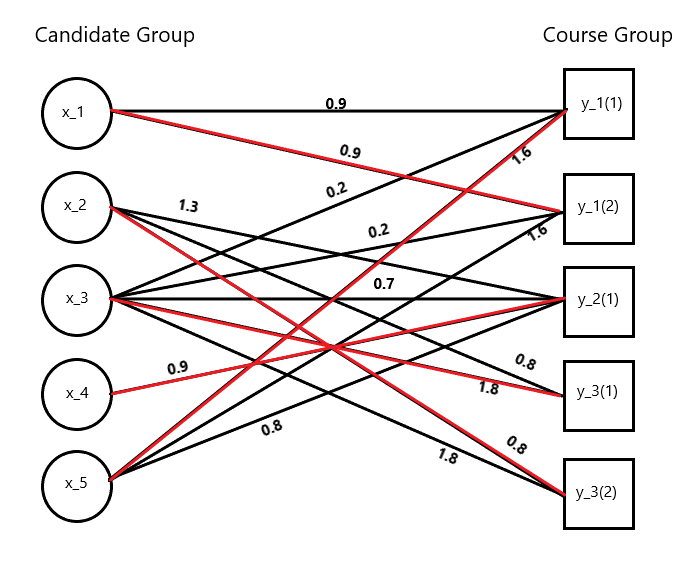
\includegraphics[width=0.5\textwidth]{MM.png}
        \caption{A sample graph including 5 candidates and 3 courses, where the $y_1$ is looking for 2 candidates, $y_2$ is looking for
        only 1 candidate, and $y_3$ also needs 2 candidates. The edge weights are the linear combination of candidate-to-course preferences and
        course-to-candidate preferences with a maximum of $\lambda_1+\lambda_2$. If not specified, $\lambda_1+\lambda_2=2$ in general. Red lines
        indicate the best assignment generated by Maximum Matching Algorithm.}
    \end{figure*}
    %------------------------------------------------
    \section{Evaluation of methods}
    \subsection{Scoring of assignments}
    In order to compare and contrast each algorithm discussed above, we will develop a "score function", which takes input
    of a produced assignment of candidates and courses, and output a numerical score, which higher score indicates better
    quality of the assignment.\\
    The input of the scoring function should be a serie of binary variables:
    $$\sigma_{i,j}=\begin{cases}1\text{, if candidate i is assigned to course j} \\
    0\text{, else}\end{cases}$$
    for each candidate $i$ and each course $j$ in the assignment.\\
    Let $m_{i, j}$ be candidate $i$'s preference score to course $j$, and $n_{j, i}$ be course $j$'s preference to candidate $i$,
    both $m$ and $n$ have value between $0$ and $1$. The return value of score function should be:
    $$\sum_i\sum_j \sigma_{i,j}(\lambda_1m_{i,j} + \lambda_2n_{j,i})$$.
    Which $\lambda_1$ and $\lambda_2$ are different weights we consider course's and candidates's preferences to the other. Currently,
    we use $1$ for both weights to value candidates and courses' opinions equally when scoring an assignment.
    All invalid assignments which breaks any of rule 1, 2, 3 in the problem description will not receive a score and should not be
    considered. (Theoretically, each algorithm described above should avoid generating an invalid assignment.)

    \subsection{Additional Metrics}
    In addition to sum the numerical preferences in the assignment, we also measure the percentage of courses and candidates which has their top-3
    requests satisfied. In more detail, in an assignment, for a matched pair (a, b), which a is candidate and b is course:
    \begin{itemize}
        \item if a's preference score for b is within the top 3 scores of all a's preference scores, we consider b is a "top-3" choice for a. Same logic
        applied to b when checking if a is a "top-3" choices for a.
        \item If there are ties: suppose there are five courses: c1, c2, c3, c4, c5, and candidate a's preference score to these courses are: 0.9, 0.8, 0.8, 0.7,
        0.6 in order, then the top 3 scores should be: 0.9, 0.8, 0.7. In this case c1, c2, c3, c4 all satisfy as "top-3" choices.
    \end{itemize}
    After getting the "top-3" satisfaction count for both candidates and courses, we calculate the satisfaction rate by:
    $$\frac{\text{number of matches satisfying "top-3"}}{\text{all matches}} \times 100\%\text{,}$$
    and "all matches" should be sum of capacity (number of candidates wanted) of all courses.
    \\ We will use both the score, and preference satisfaction rate of courses and candidates, to evaluate each method, and determine the best one.
    %------------------------------------------------
    \section{Results}
    \subsection{Simulations}
    By using \verb|Python|, we implemented the following functionalities. 
    By inputting a \verb|num_candidate| and a \verb|num_course| parameters, our program can:
    \begin{enumerate}
        \item Generate $m$ candidates and $n$ courses, which \verb|num_candidate = m| and \verb|num_course = n|.
        \item Generate random preference levels of each candidate for courses, and each course to candidates, which are
        floats between $0$ and $1$ inclusively.
        \item Generate capacity for each course, which is an integer between $1$ and $5$ inclusively.
        \item Generate qualification for each student for each course, which is an integer either $0$ or $1$, with $1$ indicates
        being qualified.
        \item Run the generated data on one (or all) of the three algorithms mentioned above.
    \end{enumerate}
    Note: for the stable-marriages method, we coded the algorithm as described in an article from Cornell University; for the Hungarian Algorithm, we
    constructed the cost matrix as defined in section 4.2, and used the \verb|scipy.optimize.linear_sum_assignment| package which exactly
    performs the Hungarian Algorithm; for the maximal matching algorithm, we used the \verb|networkx.max_weight_matching| package.
    \\ For each set of random data (includes course preference, candidate preference, capacity and qualifications) generated, we will run
    all three algorithms on it, and record the evaluations (score, preference satisfaction rate for both sides) for each method.

    \subsection{Simulation Result}
    We first start with a small sample size (50 student candidates and 5 courses) to be assigned. From Figure \ref{fig:50can_5cou}, we can see that Hungarian Algorithm and
    Maximum Matching Algorithm perform extremely well on assigning candidates to one of their top 3 choices with a mean satisfaction rate of $\approx 99.5\%$. Stable Marriage
    Algorithm is also accpetable with a mean of $80.58\%$ satisfaction rate. Considering the professors' satisfaction rate, Stable Marriage give us the best result with
    a mean of $99.49\%$ satisfaction. And Hungarian Algorithm produced assignment with an average of $\approx 81\%$ top-3 satisfied to professors, as well as Maximum Matching
    Algorithm. And for the histogram of score, we can see an interesting phenomenon that the distributions of Hungarian Algorithm and Maximum Matching Algorithm are
    exactly the same. Is that an edge case due to small sample size? We then run the simulations with a larger size (200 candidates and 15 courses).
    \\ \indent From Figure \ref{fig:200can_15cou}, we can see that the distribution of satisfaction rates becomes more dense, which is reasonable because that with
    larger data set, the model we built should have a better stability. And it is surprising that Hungarian Algorithm and Maximum Matching Algorithm perform better on 
    satisfying professors' preferences. However, the candidate satisfaction rate evalutaed from Stable Marriage Algorithm is worse than the rate we got from smaller candidate-course
    size. Furthermore, we find that the score distributions of Hungarian Algorithm and Maximum Matching Algorithm are still the same.
    \\ \indent Finally, we tested our model using relatively realistic sizes of candidates and courses (300 candidates 50 courses). We can see that Stable Marriage Algorithm
    gets a lower satisfaction rate for candidates to around $60\%$, which is not ideal. However, the other two algorithms still give back a high-stand performance that we 
    are looking for. And considering professors' preferences, all three algorithms have $100\%$ satisfaction rate. Our algorithms really make professors happy! Focusing on the 
    distribution, Stable Marriage Algorithm has a more densed distribution that is close to $100\%$ rather than other two. In fact, Maximum Matching Algorithm also lies on 
    $100\%$ satisfaction rate for professors for approximately 80 trails over 100 trails of simulation. 


    \begin{figure*}[t]
        \centering
        \begin{subfigure}{0.32\textwidth}
            \centering
            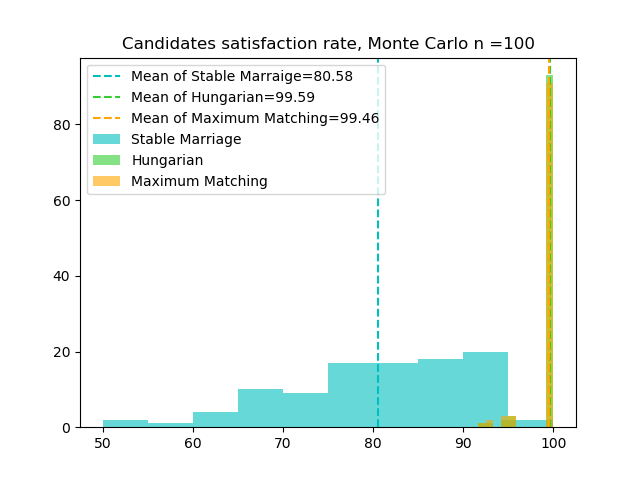
\includegraphics[width=\textwidth]{../figures/50candidates_5courses_100simulations/can_rate.png}
            \caption{Candidate Satisfaction Rate}
        \end{subfigure}%
        ~
        \begin{subfigure}{0.32\textwidth}
            \centering
            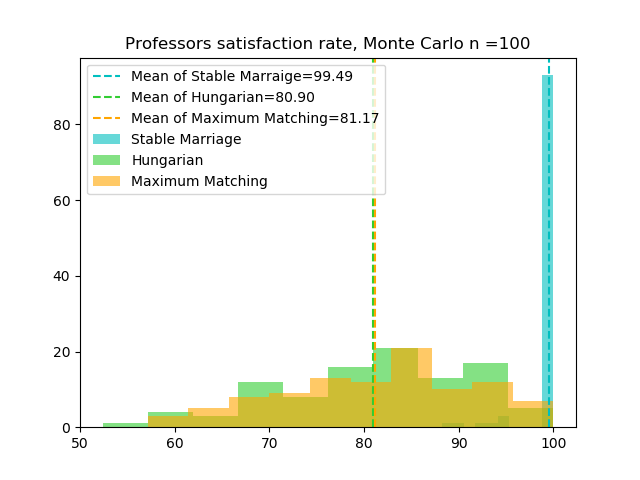
\includegraphics[width=\textwidth]{../figures/50candidates_5courses_100simulations/prof_rate.png}
            \caption{Professor Satisfaction Rate}
        \end{subfigure}
        ~
        \begin{subfigure}{0.32\textwidth}
            \centering
            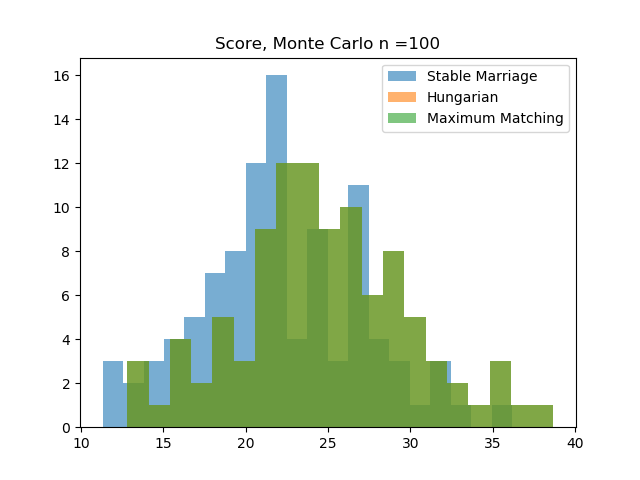
\includegraphics[width=\textwidth]{../figures/50candidates_5courses_100simulations/scores.png}
            \caption{Score}
        \end{subfigure}
        \caption{Histograms with 50 candidates and 5 courses}
        \label{fig:50can_5cou}
    \end{figure*}

    \begin{figure*}[t]
        \centering
        \begin{subfigure}{0.32\textwidth}
            \centering
            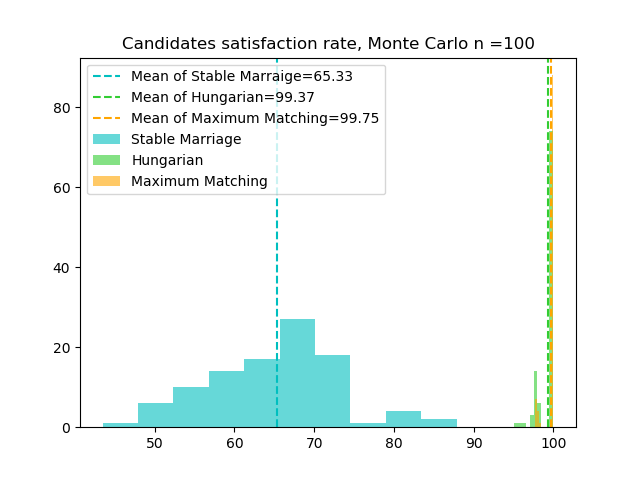
\includegraphics[width=\textwidth]{../figures/200candidates_15courses_100simulations/can_rate.png}
            \caption{Candidate Satisfaction Rate}
        \end{subfigure}%
        ~
        \begin{subfigure}{0.32\textwidth}
            \centering
            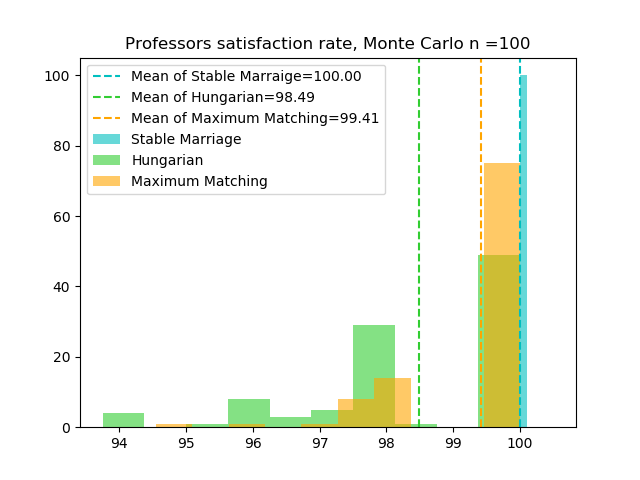
\includegraphics[width=\textwidth]{../figures/200candidates_15courses_100simulations/prof_rate.png}
            \caption{Professor Satisfaction Rate}
        \end{subfigure}
        ~
        \begin{subfigure}{0.32\textwidth}
            \centering
            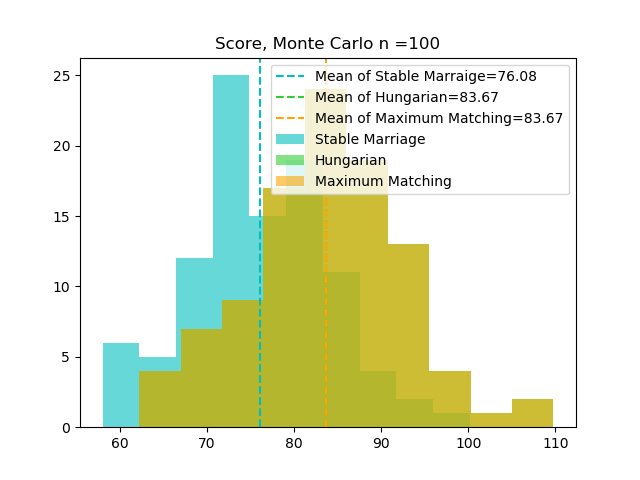
\includegraphics[width=\textwidth]{../figures/200candidates_15courses_100simulations/scores.png}
            \caption{Score}
        \end{subfigure}
        \caption{Histograms with 200 candidates and 15 courses}
        \label{fig:200can_15cou}
    \end{figure*}
    \begin{figure*}[t]
        \centering
        \begin{subfigure}{0.32\textwidth}
            \centering
            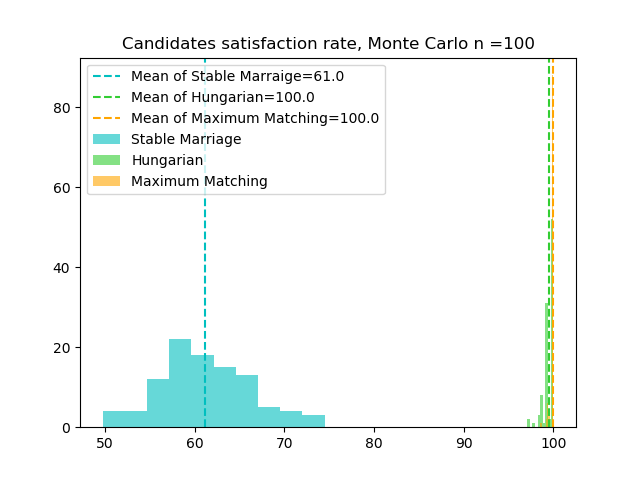
\includegraphics[width=\textwidth]{../figures/300candidates_50courses_100simulations/can_rate.png}
            \caption{Candidate Satisfaction Rate}
        \end{subfigure}%
        ~
        \begin{subfigure}{0.32\textwidth}
            \centering
            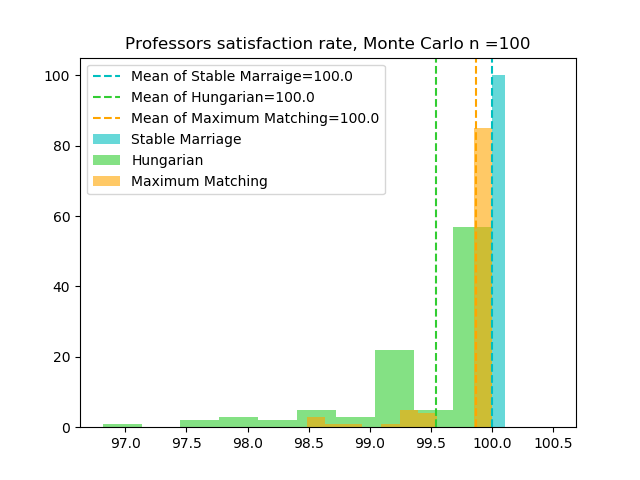
\includegraphics[width=\textwidth]{../figures/300candidates_50courses_100simulations/prof_rate.png}
            \caption{Professor Satisfaction Rate}
        \end{subfigure}
        ~
        \begin{subfigure}{0.32\textwidth}
            \centering
            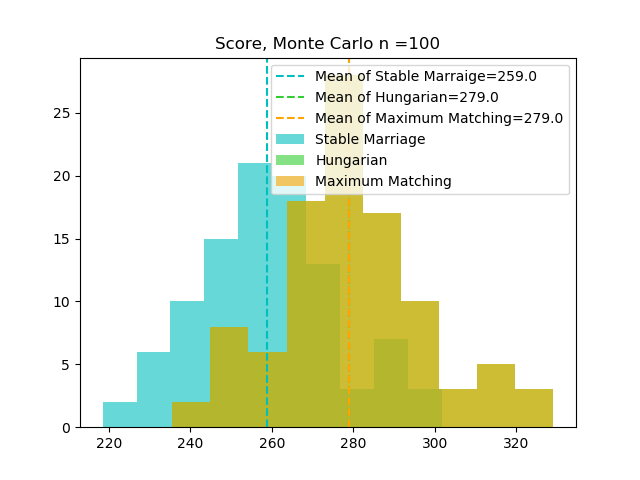
\includegraphics[width=\textwidth]{../figures/300candidates_50courses_100simulations/scores.png}
            \caption{Score}
        \end{subfigure}
        \caption{Histograms with 300 candidates and 50 courses}
        \label{fig:500can_40cou}
    \end{figure*}
    %------------------------------------------------
    \section{Conclusion}
    It is found from all sample sizes that Maximum Matching Algorithm and Hungarian Algorithm have an exactly like
    distribution of score values in the Monte Carlo simulation process with trail number $n=100$. In Maximum Matching 
    Algorithm, the "score" is $s = \lambda_1 p_{ij} + \lambda_2 p_{ji}$ which weights 
    edges connecting vertices from candidates group to courses group. In Hungarian Algorithm, the "score" is the entries
    in the cost matrix which we defined as $2 - \text{i's preference to j} - \text{j's preference to i}$. And we were 
    minimizing the cost. Therefore, they are optimizing the same score function but we implemented the score function 
    differently to fit the algorithms. So a convincing reason to the phenomena is that both Maximum Matching Algorithm and 
    Hungarian Algorithm were trying to build their assignments to maximize the same score function. 
    \\\indent In addtion, comparing the performances for different algorithms under tested sizes of candidates and courses, it could be
    safe to conclude that both Hungarian Algorithm and Maximum Matching Algorithm performs well in satisfying student candidates'
    top-3 preferences. And with the current input method (weighting professors' preferences and candidates' preferences equally), it is
    more likely that Stable Marriage Algorithm will give a best result to satisfy professors' preferneces for any data size. Meanwhile, 
    as the size of data increases, Hungarian Algorithm and Maximum Matching Algorithm will produce better assignments that also could 
    meet professors' top-3 preferences with a mean of $100\%$ probability.
    \\\indent Moreover, with the current input and evaluation method, Hungarian Algorithm and Maximum Matching will both have optimized score
    with the exact same value. On the other hand, the assignment score computed using Stable Marriage Algorithm is slightly less than the score
    retrieved from the other two methods but not far below.
    \\\indent Also, it is necessary to consider the runtime 
    %------------------------------------------------
    \section{Improvements}
    We are currently only focusing on teaching assistant posistions, but the real world problem includes more various teaching
    positions such as graders and instructors. We would also like to consider various positions for further studies.
    \\ \indent Currently we value course's preference to candidates and candidates' preference to courses equally likely. We will
    test additional weights of them. This can be achieved by
    \begin{itemize}
        \item Changing the direction of proposing in Stable Marriage Algorithm
        \item Adjusting computation of the cost matrix in Hungarian Algorithm
        \item Changing the $\lambda_1$ and $\lambda_2$ while weighting the edge in Maximum Matching Algorithm
    \end{itemize}
    We want to know the real-world implications if different weights are used.
    \\ \indent Another point to improve our method is to find out some other constraints to let our model fit the real world problem more. For example,
    we would like to construct quantification inputs instead of "qualified" or "not-qualified".
    \\ \indent Besides, if our community partners are willing to take our suggestion by chance, we would modify our input method from
    randomly generating to construct our data map using given input data such as comma-seperated-value files (.csv) and 
    SQL or NoSQL tables.
    \\ \indent In such way, I think our model could be more realistic and might be more accpetable to our community partners.
    %------------------------------------------------
    \section{References}
    [1]"The college admission problem: many-to-one matching : Networks II Course blog for INFO 4220", Blogs.cornell.edu, 2018. [Online]. 
    Available: https://blogs.cornell.edu/info4220/2016/03/18/the-college-admission-problem-many-to-one-matching/. \\

    [2]D. Gale and L. Shapley, "College Admissions and the Stability of Marriage", The American Mathematical Monthly, vol. 69, no. 1, p. 9, 1962. \\
    
    [3]"Stable Marriage Problem -- from Wolfram MathWorld", Mathworld.wolfram.com, 2018. http://mathworld.wolfram.com/StableMarriageProblem.html. \\
    
    [4]Cs.princeton.edu, 2018. [Online]. https://www.cs.princeton.edu/~wayne/kleinberg-tardos/pdf/01StableMatching.pdf. \\
    

\end{document}